% ============================================================
%  APPENDIX A — EXPERIMENT 1 FULL DETAILS
%  Place after the main body, e.g. \appendix\section{...}
% ============================================================

\section{Experiment 1: Full Experimental Details}
\label{app:exp1}

\subsection{Market Selection}
\label{app:market-selection}

We query the Polymarket REST API for all binary markets satisfying the following filters as of
June~5, 2026 (the sampling date for the pilot):

\begin{itemize}
  \item \textbf{Status}: market is open (not yet resolved or expired).
  \item \textbf{Closing window}: resolution date between 14 and 180 days from sampling date.
  \item \textbf{Volume}: CLOB transaction count $\geq 1{,}000$.
  \item \textbf{Category}: one of Politics, Government, Elections, Economics, Geopolitics.
\end{itemize}

This produces a candidate pool of 83~markets.  From these we select a pilot set of five markets
that jointly maximize category diversity (at least two distinct categories), market-price diversity
(spread across the 5--45\% range), and topic-type diversity (electoral, diplomatic, institutional).
Table~\ref{tab:markets} gives the full pilot set.

\begin{table}[h]
\centering
\caption{Pilot markets used in Experiment~1.  ``Mid'' is the Polymarket best-bid mid-price
at the time of agent elicitation (June~5--7, 2026).  $k_\text{GPT}$ and $k_\text{Claude}$
are the number of valid structured-forecast runs used in consistency analysis.}
\label{tab:markets}
\small
\begin{tabular}{p{6.2cm} l c c c}
\toprule
\textbf{Question} & \textbf{Category} & \textbf{Mid} & $k_\text{GPT}$ & $k_\text{Claude}$ \\
\midrule
Strait of Hormuz traffic returns to normal by end of June? & Geopolitics & 0.17 & 5 & 5 \\
US--Iran nuclear deal by June~30?                          & Middle East & 0.28 & 5 & 5 \\
US $\times$ Iran permanent peace deal by July~31, 2026?    & Iran        & 0.41 & 5 & 5 \\
Will Renan Santos win the 2026 Brazilian presidential election? & Brazil  & 0.16 & 5 & 5 \\
Will Tom Steyer win the California Governor Election in 2026?   & Elections & 0.22 & 5 & 5 \\
\bottomrule
\end{tabular}
\end{table}

Daily CLOB price histories for all 83~pool markets are also collected (Polymarket CLOB API,
1-day fidelity, up to 28-day rolling windows) to support calibration analysis and price-history
visualizations.

\subsection{Agent Architecture}
\label{app:agent-arch}

Both agents are deployed via Microsoft Azure AI~Foundry using the Responses~API protocol
(\texttt{client.responses.create} with \texttt{previous\_response\_id} for multi-turn
context chaining).  Web search is provided natively by the Azure AI~Foundry agent runtime;
each turn that requests research issues Bing-backed searches and receives summarized web
content before the model produces its response.

\begin{itemize}
  \item \textbf{GPT-5.4}: deployed as \texttt{forecasting-agent}, version~2; accessed at
        the Azure AI~Foundry project endpoint using the standard four-turn protocol
        (T1: event model; T2: web research; T3: deeper evidence; T4: structured JSON).
  \item \textbf{Claude Opus~4.8} (\texttt{claude-opus-4-8}): deployed as
        \texttt{forecasting-agent-2}, version~2.  Due to an Azure-side constraint that
        limits accumulated context to three chained turns before a 400-error
        (\texttt{invalid\_request\_error}), we run Claude in three-turn mode
        (T1: event model; T2: web research; T3: structured JSON), omitting the optional
        deepening turn.
\end{itemize}

Each run issues $k = 5$ independent calls with fresh context; the median yes-probability across
runs is the per-market point estimate.

\subsection{Prompting Protocol}
\label{app:prompts}

All four prompt templates are shared across agents; the structured forecast uses a fixed JSON
schema.

\paragraph{Turn 1 --- Event model and prior.}
The agent is given the market question, resolution criteria, current Polymarket mid-price, days
to resolution, and category tag.  It is asked to produce:
\begin{enumerate}
  \item A causal narrative (\textit{event model}) describing the primary mechanisms through
        which the outcome could occur or fail to occur.
  \item Two competing hypotheses: $H_1$ = yes-resolution, $H_2$ = no-resolution.
  \item For each hypothesis: a list of key actors, institutions, and latent variables; prior
        probability; and mechanistic justification for that prior.
  \item A set of \emph{information gaps}---the most important empirical questions whose
        answers would most change the forecast.
\end{enumerate}

\paragraph{Turn 2 --- Evidence gathering.}
The agent is prompted to search for time-available evidence bearing on each hypothesis, to
evaluate the direction and weight of each piece of evidence, to update its hypothesis
probabilities in light of the search results, and to note which information gaps were filled
or remain open.  The agent's web-search tool calls are logged; we record search queries and
the number of distinct searches per turn.

\paragraph{Turn 3 (GPT-5.4 only) --- Deepening.}
If any information gaps remain open after Turn~2, the agent is asked to pursue targeted
follow-up searches on the highest-priority gap and to revise its hypothesis probabilities again.

\paragraph{Final turn --- Structured JSON forecast.}
The agent is asked to consolidate all prior turns into a single structured JSON object matching
the schema below.  Parsing is attempted on the raw output; if parsing fails the run is logged
as an error and excluded from downstream analysis.

\begin{verbatim}
{
  "yes_prob": float,           // final headline probability in [0,1]
  "confidence": "low"|"medium"|"high",
  "hypotheses": [
    {
      "id": "H1",              // always H1 = yes-resolution
      "label": str,
      "prior_probability": float,
      "posterior_probability": float,
      "key_evidence": [str],
      "key_actors": [str],
      "mechanisms": [str]
    },
    { "id": "H2", ... }
  ],
  "reasoning_summary": str,
  "key_uncertainties": [str]
}
\end{verbatim}

The schema enforces the structural invariant $\hat{p} = P(H_1)$, which is tested by the ICS
metric.

\subsection{Counterfactual Packet Construction}
\label{app:cf-taxonomy}

For each market we construct nine counterfactual evidence packets, partitioned into three
directions ($3 \times 3$).  Each packet contains:

\begin{itemize}
  \item \textbf{evidence\_headline}: a short synthetic news headline (one sentence) that, if
        accepted as true, provides information with a clear causal implication for $H_1$.
  \item \textbf{mechanism\_targeted}: a one-sentence description of the causal pathway through
        which the evidence bears on the resolution outcome.
  \item \textbf{direction}: \texttt{pro\_H1} (evidence should raise $P(H_1)$),
        \texttt{anti\_H1} (evidence should lower $P(H_1)$), or \texttt{orthogonal}
        (evidence is drawn from the same domain but has no causal link to $H_1$).
  \item \textbf{slot\_type}: a label from the taxonomy in Table~\ref{tab:slot-taxonomy}.
\end{itemize}

Packets are generated using a language model prompted with the market question, the event model
produced in Stage~1, and an instruction to construct evidence that is (i)~plausible given the
resolution timeframe, (ii)~unambiguously directional, and (iii)~not already disclosed in the
agent's web-search context.  Three rounds of review are applied to each packet to confirm that
the direction label is correct.

\begin{table}[h]
\centering
\caption{Counterfactual slot-type taxonomy.  Each packet is assigned one label.}
\label{tab:slot-taxonomy}
\small
\begin{tabular}{p{3cm} p{8cm}}
\toprule
\textbf{Slot type} & \textbf{Description} \\
\midrule
DATA            & A measurement, price signal, published statistic, or poll result that
                  directly indicates the probability of $H_1$ is becoming more or less likely. \\
SIGNAL          & A statement, announcement, or observable action by a key actor that
                  provides information about their intentions or capabilities. \\
EVENT           & A discrete occurrence (meeting, vote, battle, agreement) that advances or
                  sets back the causal pathway to $H_1$. \\
PROCEDURAL      & An administrative, regulatory, or process update in the same domain that
                  has no direct causal link to whether $H_1$ or $H_2$ occurs. \\
\bottomrule
\end{tabular}
\end{table}

Table~\ref{tab:cf-example} illustrates the three directions for two of the pilot markets.

\begin{table}[h]
\centering
\caption{Representative counterfactual packets for two pilot markets.  The ``Oman'' headline
caused the largest single update in the pilot: Claude Opus~4.8 revised the Hormuz market from
10\% to 45\% ($\Delta\hat{p} = +35$~pp).}
\label{tab:cf-example}
\small
\begin{tabular}{p{2.2cm} p{1.4cm} p{5.5cm} p{3.5cm}}
\toprule
\textbf{Market} & \textbf{Direction} & \textbf{Headline} & \textbf{Mechanism} \\
\midrule
\multirow{3}{2.2cm}{Strait of Hormuz traffic returns to normal by end of June?}
  & pro-$H_1$    & Oman says Iran agrees daily protected windows for commercial Hormuz transits
                & Bilateral arrangement enables regular passage, directly raising probability of normalisation. \\
  & anti-$H_1$   & War-risk premiums for Hormuz voyages jump to new June high
                & Rising insurance costs deter transits, reducing probability of return to normal. \\
  & orthogonal   & IMO opens technical comment round on Gulf vessel incident reporting format
                & Administrative rulemaking with no causal link to Hormuz transit volumes. \\
\midrule
\multirow{3}{2.2cm}{Will Tom Steyer win the California Governor Election in 2026?}
  & pro-$H_1$    & Late mail-ballot batches narrow Steyer deficit in California governor primary
                & Remaining ballots disproportionately favour Steyer, improving his top-two finish probability. \\
  & anti-$H_1$   & Remaining California ballots concentrated in areas unfavorable to Steyer
                & Demographic concentration of uncounted votes reduces probability of Steyer overtaking Becerra. \\
  & orthogonal   & California adjusts nightly election-report posting window during routine systems maintenance
                & Administrative publication timing with no effect on vote totals or outcome. \\
\bottomrule
\end{tabular}
\end{table}

\subsection{Stage 3 Update Protocol}
\label{app:update-protocol}

Each of the nine CF packets is paired with each of the $k = 5$ initial runs for a given market
and agent, yielding 45~update records per market-agent cell.  The update prompt presents the
agent with:
\begin{enumerate}
  \item Its own Stage~1 structured forecast (JSON), including hypothesis priors and the event model.
  \item The single new counterfactual headline and its mechanism description.
  \item An instruction to (a)~reason through how the new evidence bears on each hypothesis,
        (b)~state revised posterior probabilities for $H_1$ and $H_2$, and (c)~state a
        revised final forecast.
\end{enumerate}

Web search is \emph{not} available during Stage~3.  The agent cannot verify the injected
evidence against independent sources; this is intentional, as it isolates the agent's ability
to reason from a stated premise rather than its ability to detect fabricated information.
The update prompt explicitly says the headline should be treated as true for the purposes of
the exercise.

Each update response is parsed to extract \texttt{updated\_yes\_prob} and the updated
\texttt{hypotheses[H1].posterior\_probability}.  The original Stage~1 values are stored as
\texttt{initial\_yes\_prob} and the delta $\Delta\hat{p}$ is computed as their difference.
Records with parse failures or missing fields are excluded from metric computation but logged
for error auditing (none in the pilot).

\subsection{Extended Results}
\label{app:extended-results}

\paragraph{Per-market consistency.}
Table~\ref{tab:per-market} reports the three consistency metrics broken down by market.
All per-market rates are 1.00 for both agents, indicating no market was anomalous.

\begin{table}[h]
\centering
\caption{Per-market consistency rates.  EHC and HFC apply to directional (pro/anti) updates
with $|\Delta| \geq 3$~pp; ICS applies to all 45~updates per cell.  All entries are 1.00.}
\label{tab:per-market}
\small
\begin{tabular}{p{5.5cm} l ccc cc}
\toprule
\textbf{Market} & \textbf{Model} & \textbf{EHC} & \textbf{HFC} & \textbf{ICS}
               & \textbf{Agent} $\hat{p}$ & \textbf{Market} $m$ \\
\midrule
\multirow{2}{5.5cm}{Hormuz traffic normal by Jun.~30?}
 & GPT-5.4         & 1.00 & 1.00 & 1.00 & 0.10 & \multirow{2}{*}{0.17} \\
 & Claude Opus~4.8 & 1.00 & 1.00 & 1.00 & 0.10 & \\
\midrule
\multirow{2}{5.5cm}{US--Iran nuclear deal by Jun.~30?}
 & GPT-5.4         & 1.00 & 1.00 & 1.00 & 0.22 & \multirow{2}{*}{0.28} \\
 & Claude Opus~4.8 & 1.00 & 1.00 & 1.00 & 0.11 & \\
\midrule
\multirow{2}{5.5cm}{US--Iran permanent peace deal by Jul.~31?}
 & GPT-5.4         & 1.00 & 1.00 & 1.00 & 0.07 & \multirow{2}{*}{0.41} \\
 & Claude Opus~4.8 & 1.00 & 1.00 & 1.00 & 0.05 & \\
\midrule
\multirow{2}{5.5cm}{Renan Santos wins 2026 Brazil presidential election?}
 & GPT-5.4         & 1.00 & 1.00 & 1.00 & 0.03 & \multirow{2}{*}{0.16} \\
 & Claude Opus~4.8 & 1.00 & 1.00 & 1.00 & 0.01 & \\
\midrule
\multirow{2}{5.5cm}{Tom Steyer wins 2026 California Governor race?}
 & GPT-5.4         & 1.00 & 1.00 & 1.00 & 0.01 & \multirow{2}{*}{0.22} \\
 & Claude Opus~4.8 & 1.00 & 1.00 & 1.00 & 0.10 & \\
\bottomrule
\end{tabular}
\end{table}

\paragraph{Per-direction revision magnitudes.}
Table~\ref{tab:anchoring} reports mean absolute forecast revision $\overline{|\Delta\hat{p}|}$
by CF direction, replicated from the standalone evaluation script.  Pro-$H_1$ updates produce
the largest absolute revisions for both agents, anti-$H_1$ updates produce moderate revisions,
and orthogonal updates produce revisions close to zero.  The asymmetry between pro and anti
magnitudes ($11.3$~pp vs.\ $4.8$~pp for Claude; $8.4$~pp vs.\ $3.6$~pp for GPT) is consistent
with the lower end of the prior distribution for these markets: upward revisions from low priors
can travel further in absolute terms than downward revisions that are already near zero.

\begin{table}[h]
\centering
\caption{Mean absolute forecast revision $\overline{|\Delta\hat{p}|}$ by counterfactual direction.
SE in parentheses.  The \emph{sensitivity ratio} is $\overline{|\Delta\hat{p}|}_{\text{pro+anti}}
/ \overline{|\Delta\hat{p}|}_{\text{ortho}}$.}
\label{tab:anchoring}
\begin{tabular}{lcccc}
\toprule
\textbf{Model} & pro-$H_1$ & anti-$H_1$ & orthogonal & \textbf{Sensitivity} \\
\midrule
GPT-5.4         & 8.4~pp (0.6) & 3.6~pp (0.3) & 0.71~pp (0.08) & $8.5\times$ \\
Claude Opus~4.8 & 11.3~pp (1.0) & 4.8~pp (0.4) & 0.23~pp (0.05) & $34.6\times$ \\
\bottomrule
\end{tabular}
\end{table}

\paragraph{Inter-run variation.}
Across $k = 5$ runs per market per model, the inter-run standard deviation of the initial
yes-probability was $\leq 2$~pp for GPT-5.4 and $\leq 4$~pp for Claude Opus~4.8 on most
markets (the Steyer market showed slightly higher variance, $\sigma \approx 3$~pp for Claude).
This indicates that the structured-forecast elicitation is stable across independent runs:
the agents arrive at similar initial probability estimates even without information sharing
between runs.

\subsection{Limitations and Future Directions}
\label{app:exp1-limitations}

\paragraph{Sample size.}
The pilot comprises five markets and two agents, yielding 315~update records in total.  The
ceiling effects on EHC, HFC, and ICS (all $= 1.00$) preclude any within-sample ranking of
models on consistency quality, and the small market sample makes it impossible to detect
heterogeneity across market types or domains.  The full experiment targets at least 100~markets
as specified in the original protocol.

\paragraph{CF difficulty.}
All counterfactual packets in the pilot were designed to be unambiguous: the direction of
implication was meant to be clear to any informed reader.  It is possible that both agents pass
these consistency checks not because they have coherent world models but because the evidence
headlines are so direct that any agent pattern-matching on lexical cues (``war-risk premiums
jump'' $\to$ bad for normalisation) would pass.  Future work should include CFs where the
mechanism is indirect, where a pro-$H_1$ headline has anti-$H_2$ content that is easy to
confuse, or where the evidence bears on a latent variable whose connection to the hypothesis
requires multi-step inference.

\paragraph{No-evidence control.}
The orthogonal packets serve as a partial no-evidence control, but they are not strictly
equivalent to presenting no evidence at all.  A stronger test would ask the same agent to
produce an update given literally no new information, to confirm that the baseline revision
rate is near zero.  In the pilot, Claude Opus~4.8's orthogonal mean revision is $0.23$~pp,
which is near-zero and supports the interpretation, but this control should be formalised in
the full experiment.

\paragraph{Stage 3 verifiability.}
Because Stage~3 updates are run without web search, agents cannot verify the injected
headlines.  An agent with access to web search might flag the synthetic headline as
unverifiable and refuse to update strongly on it.  This would represent sensible epistemic
caution rather than a consistency failure, but it would reduce the observable EHC and HFC
rates.  The full experiment should include conditions both with and without web access at
Stage~3 to disentangle verifiability from consistency.

\paragraph{Resolution outcomes.}
At the time of writing, none of the five pilot markets have resolved.  When they do, we will
be able to compute calibration scores (Brier score, log loss) and ask whether the agents'
pre-update forecasts are better or worse calibrated than Polymarket prices, and whether
the direction of agent-market divergence is predictive of resolution outcome.

% ============================================================
%  FIGURE GENERATION CODE (pgfplots)
%  Save as figures/exp1_results.tex and compile separately,
%  or \input{} directly if pdflatex is used.
% ============================================================

\subsection{Figure Generation Code}
\label{app:fig-code}

The center panel of Figure~\ref{fig:exp1-results} is produced by the following
\texttt{pgfplots} code.

\begin{verbatim}
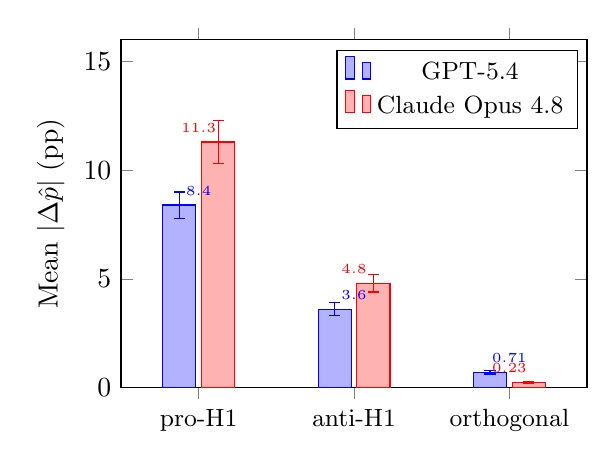
\begin{tikzpicture}
\begin{axis}[
  ybar, bar width=12pt, width=7.5cm, height=6cm,
  symbolic x coords={pro-H1, anti-H1, orthogonal},
  xtick=data, xticklabel style={font=\small},
  ylabel={Mean $|\Delta\hat{p}|$ (pp)},
  ymin=0, ymax=16,
  legend style={at={(0.98,0.97)}, anchor=north east, font=\small},
  enlarge x limits=0.25,
  error bars/y dir=both, error bars/y explicit,
  nodes near coords, nodes near coords align={vertical},
  every node near coord/.style={font=\tiny},
]
%% GPT-5.4
\addplot+[error bars/.cd, y dir=both, y explicit]
  coordinates {
    (pro-H1,   8.4) +- (0,0.6)
    (anti-H1,  3.6) +- (0,0.3)
    (orthogonal, 0.71) +- (0,0.08)
  };
%% Claude Opus 4.8
\addplot+[error bars/.cd, y dir=both, y explicit]
  coordinates {
    (pro-H1,   11.3) +- (0,1.0)
    (anti-H1,   4.8) +- (0,0.4)
    (orthogonal, 0.23) +- (0,0.05)
  };
\legend{GPT-5.4, Claude Opus 4.8}
\end{axis}
\end{tikzpicture}
\end{verbatim}
